\documentclass[11pt,a4paper]{article}
\usepackage[margin=2.3cm]{geometry}
\usepackage[T1]{fontenc}
\usepackage{lmodern,microtype,amsmath,amssymb,amsthm,booktabs,array,tabularx,graphicx}
\usepackage{enumitem,algorithm,algpseudocode,xcolor,listings}
\usepackage[numbers,sort&compress]{natbib}
\usepackage[colorlinks=true,linkcolor=blue!50!black,citecolor=blue!50!black,urlcolor=blue!50!black]{hyperref}
\hypersetup{pdftitle={Rotating Group Assignments with a Companion Guarantee},pdfauthor={Isaac Lin},pdfsubject={Structural limits, auditable screening, and a hybrid solver},pdfkeywords={group assignment, companion guarantee, constraint programming, privacy inference}}
\usepackage{xurl,caption}
\usepackage[section]{placeins}
\graphicspath{{figures/}}
\setlength{\emergencystretch}{2em}
\newtheorem{theorem}{Theorem}
\newtheorem{proposition}[theorem]{Proposition}
\newtheorem{lemma}[theorem]{Lemma}
\theoremstyle{definition}\newtheorem{definition}[theorem]{Definition}
\theoremstyle{remark}\newtheorem{remark}[theorem]{Remark}
% Study macros derive from verified full traces; Bench macros use the separately disclosed exploratory summary.
\newcommand{\HonestExactlyOne}{99.73}
\newcommand{\HonestExactlyOneMin}{98.83}
\newcommand{\HonestMet}{74.48}
\newcommand{\RandomMet}{72.31}
\newcommand{\RandomMetExpected}{72.29}
\newcommand{\RandomMetExpectedAllMixed}{74.72}
\newcommand{\RandomGeOneExpected}{21.85}
\newcommand{\RandomGeOneExpectedMixed}{16.05}
\newcommand{\RandomGeOneExpectedSame}{27.65}
\newcommand{\SeedDiffCILow}{2.27}
\newcommand{\SeedDiffCIHigh}{2.67}
\newcommand{\NSeeds}{10}
\newcommand{\Seed}{7}
\newcommand{\SeedExactlyOneMean}{99.67}
\newcommand{\SeedExactlyOneMin}{99.54}
\newcommand{\SeedExactlyOneMax}{99.83}
\newcommand{\SeedDiffMean}{+2.46}
\newcommand{\SeedDiffMin}{+2.07}
\newcommand{\SeedDiffMax}{+2.99}
\newcommand{\LeakForced}{618}
\newcommand{\LeakEdges}{2056}
\newcommand{\LeakCorrect}{618}
\newcommand{\LeakStudents}{240}
\newcommand{\LeakFraction}{30.1}
\newcommand{\LeakFull}{0}
\newcommand{\FairMin}{67}
\newcommand{\FairMax}{84}
\newcommand{\FairLowIn}{75.55}
\newcommand{\FairHighIn}{72.50}
\newcommand{\NoneIntact}{16}
\newcommand{\NoneAvgCluster}{6.00}
\newcommand{\StarIntact}{0}
\newcommand{\StarAvgCluster}{3.00}
\newcommand{\StratIntact}{8}
\newcommand{\StratAvgCluster}{3.71}
\newcommand{\ScreenedIntact}{0}
\newcommand{\ScreenedAvgCluster}{3.00}
\newcommand{\StarPatterns}{3+3 in 16 rotations}
\newcommand{\StratIntactSame}{8}
\newcommand{\StratIntactMixed}{0}
\newcommand{\SharedIntactSame}{8}
\newcommand{\SharedReturned}{7}
\newcommand{\StarBound}{3}
\newcommand{\StarBoundWirings}{30}
\newcommand{\RepeatsWorseCount}{2}
\newcommand{\RepeatsWorseRotations}{3, 5}
\newcommand{\IsolatedExactlyOne}{89.59}
\newcommand{\IsolatedMeanList}{7.07}
\newcommand{\LongLeakForced}{1648}
\newcommand{\LongLeakFraction}{80.2}
\newcommand{\LongLeakFull}{69}
\newcommand{\NonSubmitters}{0}
\newcommand{\RejectedByRules}{0}
\newcommand{\MaxSolve}{53.8}
\newcommand{\Workers}{8}
\newcommand{\CpsatTime}{3.5}
\newcommand{\AnnealIters}{300\,000}
\newcommand{\Versions}{Python 3.14.7, NumPy 2.5.2, OR-Tools 9.15.6755}
\newcommand{\PrimaryRotations}{320}
\newcommand{\ReleaseOptimized}{320}
\newcommand{\ReleaseIncumbent}{0}
\newcommand{\ReleaseFallback}{0}
\newcommand{\ProvenOptimalRotations}{10}
\newcommand{\CpsatAcceptedRotations}{320}
\newcommand{\CpsatFeasibleRotations}{320}
\newcommand{\CpsatPairVarsMax}{9145}
\newcommand{\CpsatConstraintsMax}{374\,954}
\newcommand{\CpsatMeanSeconds}{10.3}
\newcommand{\MeanSolveSeconds}{18.3}
\newcommand{\ConstructionInfeasibleRotations}{65}
\newcommand{\PeersMin}{67}
\newcommand{\PeersPTen}{70.0}
\newcommand{\PeersMedian}{74.0}
\newcommand{\PeersMinRandom}{62}
\newcommand{\PeersPTenRandom}{68.0}
\newcommand{\RepeatSameMedian}{4.0}
\newcommand{\RepeatSameMax}{8}
\newcommand{\ConcentrationMedian}{25}
\newcommand{\ExtrasPerObligatedRotation}{0.0027}
\newcommand{\ExactlyOneObligated}{99.73}
\newcommand{\PendingReview}{0}
\newcommand{\ApprovedExceptions}{0}
\newcommand{\VoluntaryNonsubmission}{0}
\newcommand{\ObligatedStudents}{257}
\newcommand{\ExposureTopOne}{98.0}
\newcommand{\ExposureTopOneRandom}{3.5}
\newcommand{\ExposureTopThree}{84.0}
\newcommand{\CurrentOnlyForced}{0}
\newcommand{\FullModelExamined}{0}
\newcommand{\ScreenedFullModelForced}{0}
\newcommand{\ScreenedFullModelExamined}{10}
\newcommand{\SourceHash}{e1a4d21af6c3}
\newcommand{\BenchRotations}{10}
\newcommand{\BenchExactMeanSeconds}{5.0}
\newcommand{\BenchExactMaxSeconds}{7.3}
\newcommand{\BenchSurrogateMeanSeconds}{3.6}
\newcommand{\BenchExactWorsened}{0}
\newcommand{\BenchExactImproved}{9}
\newcommand{\BenchSurrogateWorsened}{7}
\newcommand{\BenchPreviousCountWorsened}{8}
\newcommand{\BenchMaxHistoryPairs}{5758}
\newcommand{\BenchAnnealIters}{100\,000}
\newcommand{\VerifiedAttempts}{35}
\newcommand{\VerifiedRuns}{32}
\newcommand{\VerifiedRotations}{517}

% User-provided affiliation labels; full SMU name and disclosures await confirmation.
\newcommand{\AuthorAffiliations}{MIT Lincoln Laboratory; SMU}
\newcommand{\FundingDeclaration}{Funding information has not yet been confirmed by the author and must be completed before submission.}
\newcommand{\ConflictDeclaration}{The author has not yet confirmed a competing-interest declaration; this statement must be completed before submission.}

\title{Rotating Group Assignments with a Companion Guarantee:\\Structural Limits, Auditable Screening, and a Hybrid Solver}
\author{Isaac Lin\\\small \AuthorAffiliations}
\date{Audited manuscript draft, 13 September 2026}
\begin{document}
\maketitle
\begin{abstract}
Repeated group assignment can combine a familiar companion with opportunities to meet other participants. A hard guarantee that each submitter shares a group with at least one named peer, however, can also enable coordinated submissions to force a coalition together. We formalize this directed-list assignment problem with capacities, eligibility states, attendance, administrator constraints, and two kinds of meeting history. We establish NP-completeness of its feasibility problem with unrestricted list lengths and distinguish structural forcing from global feasibility. An explicit seven-person cycle with a shared outside anchor defeats closure-only screening. We introduce a sound, bounded screening procedure that tests whether a candidate core can be separated after relaxing outside obligations, and a full-model separation test that decides, under the complete current constraints, whether a candidate group can occupy two tables; inconclusive solver outcomes remain unresolved. Submissions carry explicit states, so a short list is a visible request rather than a silent nonsubmission, and a present participant with no present eligible companion is an explicit conflict. A hybrid method combines construction, repair, simulated annealing, and constraint programming on one canonical objective, with independently validated feasibility witnesses retained as fallbacks so that a failed or time-limited optimization can still release a valid chart when a valid fallback exists. In a synthetic case study with 257 participants and alternating eligibility states, \NSeeds\ paired population seeds yield a mean exactly-one-listed-peer rate of \SeedExactlyOneMean\% and a mean increase of \SeedDiffMean\ distinct peers over a capacity-matched random baseline after 16 assignments; \ReleaseFallback\ of \PrimaryRotations\ primary rotations released a fallback chart. An incomplete method-comparison grid against a companion-preserving construction-and-repair baseline includes retained attempts with short and concentrated lists, nonsubmission and approved exceptions, absences, coalitions, and infeasible and time-limited inputs. Published charts reveal preferences: under a public list-size cap, \LeakFraction\% of submitted directed entries are logically forced in the reference run, and the most frequent tablemate of an obligated participant is a listed peer for \ExposureTopOne\% of participants using recurrence counts across the observed rotations without a public cap. Full traces, an attempt ledger, independent checks, and an interactive playback accompany the study. The procedure does not establish complete resistance to coordinated submissions, feasibility of every admitted input, confidentiality of preferences, or psychological and distributive benefits in a real population.
\end{abstract}
\noindent\textbf{Keywords:} group assignment; directed preferences; constraint programming; simulated annealing; strategic submissions; privacy inference

\section{Introduction}
A rotating lunch assignment has two potentially competing aims: give participants access to a familiar peer and create contact beyond an established circle. We study a concrete operational version of these aims. A participant may submit a list of acceptable companions, and every released assignment must place that participant with at least one present, eligible listed peer. Among assignments satisfying this requirement, the procedure discourages additional listed peers and repeated meetings. A declared acceptable companion is an input to an optimization problem; the model does not establish friendship quality, emotional security, or improved belonging.

The guarantee changes the strategic possibilities. A directed cycle of one-name lists forces its members to remain together. Increasing a minimum list length is insufficient when some names become ineligible in a particular rotation, and even two eligible names can force a group through a shared outside anchor. Rejecting every unusual list structure is also unjustified: structural dependence can arise from sincere preferences. An operational system therefore needs explicit proof conditions, an honest account of screening coverage, and a procedure for unresolved submissions. It also needs explicit handling of the ordinary frictions of a school: lists that fail a submission rule, absent companions, seats reserved by staff, and optimization runs that fail or time out.

This paper makes four contributions. First, it specifies the assignment and history objectives precisely, in one canonical form used by every stage, and proves a general feasibility hardness result. Second, it develops structural counterexamples, a sound relaxation for detecting forced candidate cores, capacity-demand tests, and a full-model separation test with three interpreted outcomes. Third, it documents a working hybrid implementation with explicit submission states, attendance-aware rosters, staff constraints, validated fallback charts, and independently checkable final and intermediate stages. Fourth, it evaluates that implementation on a reproducible synthetic study, including a companion-preserving baseline, coordinated submissions, computational budgets, network structure, attendance, and information revealed by released charts. The accompanying website replays actual saved solver stages; it does not claim to optimize a new instance in the browser.

\section{Related work}
Practical seating optimization has been studied with application-specific objectives and local search \citep{lewis2016seating}. Work on optimal seat arrangement analyzes how preference and seating graph structure affect computational complexity \citep{ceylan2023seat}. Our feasible sets differ because a directed acceptable-companion condition is mandatory, groups have exact occupancy targets, eligibility and attendance change across rotations, and past meetings affect the objective. The social golfer problem provides a related repeated-grouping model focused on avoiding repeated pairs \citep{dotu2005golfers}. Here repeated listed companionship is sometimes unavoidable: with a fixed list of at most eight names and 16 guaranteed assignments, a submitter must repeat a listed companion.

The feasibility reduction uses the graph-factor framework of \citet{kirkpatrick1983factor}. The structural analysis connects to vertex-disjoint directed cycles \citep{thomassen1983} and partitions of directed graphs under degree conditions \citep{alon2006splitting}. Alon's directly related \emph{High School Coalitions} note studies the same one-listed-companion condition without the present capacities and changing eligibility states \citep{aloncoalitions}. It already uses the cycle-extension argument and distinguishes the strategic possibilities with two versus three names. We treat these arguments as prior results. Our contribution is their application to state-dependent assignment, an auditable targeted separation test, and the evaluated implementation; we do not claim the general coalition phenomenon as new. The optimization stages use the Metropolis acceptance rule and simulated annealing \citep{metropolis1953,kirkpatrick1983annealing}, followed by OR-Tools CP-SAT \citep{ortools}. Its status distinctions are essential: UNKNOWN establishes neither feasibility nor infeasibility \citep{cpsatstatus}.

\section{Model, submissions, and objective}\label{sec:model}
Let $V$ be a set of $N$ participants. Rotation $r$ assigns each present participant to exactly one table in $\mathcal T_r$. Each table has a physical capacity $c_t$ and an occupancy target $o_t\le c_t$, and the targets sum to the number of present participants; absences reduce targets one seat at a time, largest tables first within the admissible eligibility pool. An eligibility state may restrict a table to a grade or other block. Administrators may declare prohibited pairs, which never share a table, and placement restrictions, which limit a participant to certain tables.

\subsection{Submission states}
Let $L_i\subseteq V\setminus\{i\}$ be participant $i$'s submitted list. Under the defended submission policy, a compliant list contains at least four distinct names, including two same-grade names, and at most eight. Each submission is in exactly one state: \emph{accepted}; \emph{pending review}, a nonempty list that fails the rule and is held as a visible request; \emph{approved exception}, a reviewed short list that keeps its actual obligation; or \emph{voluntary nonsubmission}. Pending requests block scheduling until an administrator approves, asks for a resubmission, or records a withdrawal. The system never pads a list or converts a failing list into nonsubmission on its own; a simulation policy that applies one decision to every pending request is recorded as such. Let $U$ be the set of obligated participants (accepted or approved). Participation and admission counts are reported separately from guarantee satisfaction, so that exclusions cannot improve coverage. The minimum-name rules do not imply global feasibility. List entries are directed: $j\in L_i$ need not imply $i\in L_j$.

\subsection{Guarantee, attendance, and conflicts}
Let $V_r$ be the present roster and let $W_r\subseteq U\cap V_r$ contain participants with an explicitly recorded waiver. The active obligations are $U_r=(U\cap V_r)\setminus W_r$. Filtering the list for rotation $r$ by eligibility and presence gives $L_i^{(r)}$. If $t_r(i)$ denotes the assigned table, define
\begin{equation}
 s_i^{(r)}=\left|L_i^{(r)}\cap\{j:t_r(j)=t_r(i)\}\right|.
\end{equation}
A valid chart respects eligibility, occupancy targets, prohibited pairs and placement restrictions and satisfies
\begin{equation}\label{eq:guarantee}
 s_i^{(r)}\ge1\qquad(i\in U_r).
\end{equation}
A present obligated participant whose every listed name is absent or ineligible has $L_i^{(r)}=\varnothing$; this is an explicit conflict that stops scheduling until an administrator records a decision for that rotation (a waiver, a list change through review, or a change of attendance). The obligation is never dropped silently, and a waiver is recorded in the released trace.

\subsection{One canonical objective}
For an unordered pair $\{a,b\}$, let $m_{ab}^{(r)}$ count prior incidental meetings, at which neither participant listed the other, and let $\alpha_{ab}^{(r)}$ count prior meetings at which at least one listed the other. Each meeting contributes to exactly one counter. The objective for rotation $r$ is
\begin{equation}\label{eq:cost}
 C_r=w_e\sum_{i\in U_r}\max(0,s_i^{(r)}-1)
 +\lambda\sum_{\{a,b\}\subseteq V_r:t_r(a)=t_r(b)}\left(5m_{ab}^{(r)}+2\alpha_{ab}^{(r)}\right),\quad\lambda=0.1,
\end{equation}
with a configurable penalty $w_e$ per additional listed companion (default $w_e=1$). The first term counts extra listed peers, not merely participants with two or more peers. The second penalizes repeated incidental meetings more strongly than repeated listed companionship. The hard requirement \eqref{eq:guarantee} is not a weight and is not configurable. Every objective weight is nonnegative and rational; the implementation uses the smallest integer scale $s$ that makes every scaled weight integral ($s=10$ for the defaults) and adds $1000s$ per violated hard constraint during search only. All optimization stages evaluate the same objective $sC_r$ over valid charts. Construction and repair are feasibility heuristics; neither they nor bounded annealing are claimed to attain its minimum. The default constraint-programming model uses this exact objective rather than a separate surrogate.

\subsection{Scheduling outcomes}
A run ends in exactly one of four outcomes: \emph{scheduled}, every rotation released an independently validated chart; \emph{review required}, pending requests, screen returns, unresolved checks, rule violations without an approved exception, or attendance conflicts need a decision; \emph{proven infeasible}, CP-SAT proved a state infeasible or a direct hard-constraint contradiction established impossibility; or \emph{unknown}, bounded search found no valid chart and no validated fallback existed, which is not a proof. Within a scheduled year each rotation carries a release status (Section~\ref{sec:fallback}).

\section{Feasibility and structural limits}
\subsection{General computational complexity}
\begin{theorem}\label{thm:hard}
In the generalized model with unrestricted list lengths, deciding whether a valid single-rotation chart exists is NP-complete, even with one eligibility block, every capacity and occupancy target equal to three, mutual lists, and every participant present and obligated with a nonempty list.
\end{theorem}
\begin{proof}
Membership in NP follows by checking a proposed chart. Reduce from $P_3$-factor, the NP-complete problem of partitioning the vertices of an undirected graph into three-vertex paths \citep{kirkpatrick1983factor}. If the source graph has an isolated vertex or its order is not divisible by three, its answer is NO. Map it to a fixed NO assignment instance: the six vertices of a star $K_{1,5}$, mutual neighbor lists, and two tables of size three. Every leaf must sit with the center, which is impossible.

Otherwise create one participant per source vertex, make every graph edge a mutual list relation, and use tables of size three. Every list is nonempty. A source $P_3$-factor supplies a chart in which every participant has a listed tablemate. Conversely, each valid three-person table induces a graph with no isolated vertex. Such a graph is a path or a triangle and contains a spanning $P_3$. Selecting one path per table gives the required factor. The construction is polynomial.
\end{proof}
The preprocessing matters because an isolated source vertex would otherwise become a nonsubmitter with no obligation. The reduction makes every constructed participant obligated independently of the admission policy and allows lists longer than eight. It proves hardness for unrestricted lists, not for the defended four-to-eight-name policy or the six-or-seven-seat instances studied below.

\subsection{Closed sets and forcing}
Throughout the following fixed-state arguments, $V$, $U$, and $L_i$ abbreviate the present roster $V_r$, active obligations $U_r$, and effective lists $L_i^{(r)}$. All forcing claims are conditional on a valid chart existing.
\begin{definition}
A set $S\subseteq V$ is \emph{guarantee-closed} in a fixed state if every $i\in S\cap U$ has at least one eligible listed peer in $S$. It is \emph{self-contained} if every eligible name of each such $i$ lies in $S$. A self-contained set is \emph{structurally coercive} if it admits no partition into two guarantee-closed parts each containing a submitter.
\end{definition}
Guarantee-closed means at least one internal acceptable peer, whereas self-contained means all acceptable peers remain inside. The forcing and demand arguments below require the latter condition.

\begin{proposition}\label{prop:forcing}
All submitters of a self-contained structurally coercive set must share a table in every valid chart.
\end{proposition}
\begin{proof}
Intersect the set with each occupied table of a valid chart. Self-containment and the guarantee make each nonempty intersection guarantee-closed. If submitters occupy at least two tables, one intersection and the union of the others form a forbidden two-part partition.
\end{proof}
This is a sufficient forcing certificate, not a global feasibility certificate. A noncoercive set may still be impossible to place because of capacities or other participants' obligations. Likewise, the ability to fit a forced group at one table does not certify the remaining population.

\begin{proposition}\label{prop:three}
A self-contained set $S$ with $S\cap U\ne\varnothing$ is not structurally coercive if every vertex of $S\cap U$ has at least three distinct eligible out-neighbors in $S\cap U$.
\end{proposition}
\begin{proof}
The minimum-outdegree-three theorem gives two vertex-disjoint directed cycles \citep{thomassen1983}. We use the extension argument described by Alon \citep{aloncoalitions}, adapted to the obligated subgraph. Start with the two cycles as separate guarantee-closed sets. Repeatedly attach any remaining obligated vertex with an edge into an existing set. When no attachment is possible, every remaining obligated vertex has all its obligated out-neighbors among the remaining vertices; their union is guarantee-closed and can be merged into the first set. Non-obligated vertices can be assigned freely. Both sets still contain their original cycle.
\end{proof}
Three arbitrary names do not meet this hypothesis if some become ineligible or are outside the obligated subgraph. The implementation applies the shortcut only when all tested vertices have obligations and counts distinct neighbors.

\subsection{Coordinated submissions and the shared-anchor counterexample}
For odd $g\ge3$, the directed circulant with edges $i\to i+1$ and $i\to i+2$ modulo $g$ is structurally coercive. Any directed cycle contains at least $\lceil g/2\rceil$ vertices: its positive steps sum to a multiple of $g$ and each step is at most two. Two disjoint cycles are therefore impossible. Two nonempty guarantee-closed parts would each contain a directed cycle, giving a contradiction. For even $g\ge4$, the two parity classes instead provide a split.

Eligibility permits this construction despite a four-name minimum. Seven same-grade participants can list their next two coalition members and two participants from the other grade. In a same-grade rotation the last two names disappear, forcing the seven together. A related six-person attack uses an odd five-person core and a sixth participant dependent on it.

\begin{proposition}\label{prop:shared}
For $g\ge2$, let a coalition $C=\{v_0,\ldots,v_{g-1}\}\subseteq U$ of present, obligated participants have effective lists $L_{v_i}=\{v_{i+1\bmod g},h\}$ for a common present outside anchor $h\in V\setminus C$. Every valid chart seats all members of $C$ together, regardless of $h$'s list.
\end{proposition}
\begin{proof}
A table containing a coalition member but not $h$ must contain that member's successor and, inductively, the entire cycle. If the coalition occupied two tables, at least one would exclude $h$, so that table would already contain the whole coalition, a contradiction.
\end{proof}
For $g=7$ and maximum capacity seven, the coalition captures a full table and $h$ sits elsewhere. Adding two opposite-grade names to each list satisfies the four-name rule while preserving the same-grade argument. A successor closure that follows $h$'s outgoing names can become very large. Even an unbounded test of that larger closure can find a split separating the intact coalition from the background without separating any coalition members. Closure size alone is therefore not the complete problem.

\begin{figure}[tb]\centering
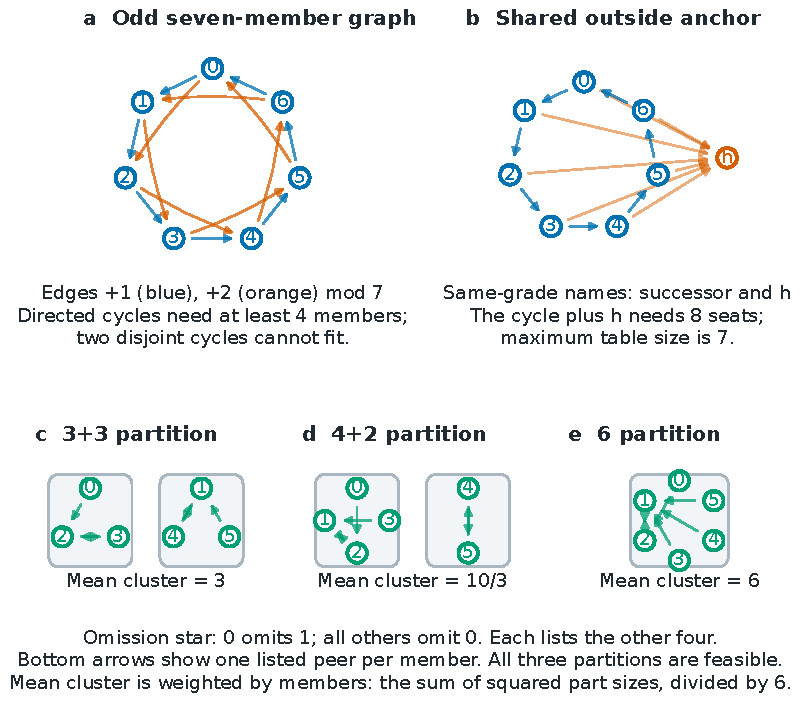
\includegraphics[width=\linewidth]{structural_examples.pdf}
\caption{Structural examples. The odd circulant and shared-anchor cycle force their cores together. In the six-person omission-star wiring, a feasible partition can be $3+3$, $4+2$, or $6$. A lower bound of three on member-weighted cluster size does not force exactly two triples or prevent an intact assignment.}\label{fig:structures}
\end{figure}

\subsection{A sound targeted-core relaxation}\label{sec:screen}
Choose a candidate $C\subseteq U$ and let $B=(\bigcup_{i\in C}L_i)\setminus C$. On $C\cup B$, retain every original outgoing name of each member of $C$, while removing all obligations of $B$. Test whether this relaxed system has a guarantee-closed bipartition with a member of $C$ on each side.
\begin{proposition}\label{prop:target}
If no such relaxed bipartition exists, every valid original chart places all of $C$ together.
\end{proposition}
\begin{proof}
Any original chart separating two core members induces a partition of $C\cup B$ by tables. Every core member retains its actual supporting edge in this restriction, since all its outgoing names were included. Outside vertices have no obligations in the relaxation. Merge the table parts into two groups, retaining a core member in each. The result is a relaxed guarantee-closed bipartition, contradicting the test outcome.
\end{proof}
A found split clears this necessary test only; it need not extend to a valid chart with the original outside obligations and physical capacities. Outside anchors are not themselves returned merely because they occur in a forcing certificate for the core.

Structural admission screening uses the full submitted roster in each requested eligibility state; it does not recompute its candidate graph after every absence or waiver. It can therefore request review even when a particular attendance-restricted schedule is feasible. The implementation enumerates successor closures of at most 64 vertices and strongly connected cores of sizes 2--12 in the original directed graph and in graphs formed by deleting one vertex. Candidates are deduplicated, sorted by size and identifiers, and limited to 256 targeted cores. Deleted-anchor edges are restored before testing. Relaxations with at most 20 vertices are exhaustively checked; larger ones use CP-SAT with a deterministic-time budget of 10, one worker, and seed zero. Each candidate receives one of three outcomes: proved separable under the test, proved coercive, or unresolved. UNKNOWN is unresolved and never triggers an automatic coercion return. All budgets are configurable, and every report records how many candidates were discovered, examined, and skipped. This candidate family is intentionally bounded and is not a complete anti-capture algorithm.

\subsection{Full-model separation tests}\label{sec:fullmodel}
The relaxation incorporates presence and eligibility through the effective lists but ignores capacities, staff constraints, and other participants' obligations. For high-risk candidates (unresolved, proved coercive, or exposed only after deleting an anchor) and for any group an administrator names, the implementation also asks the complete model of the rotation state. Let $x_{it}$ be the assignment variables of Section~\ref{sec:cp} with every hard constraint of the current inputs. For a candidate group $C$, add
\begin{equation}\label{eq:separation}
 \sum_{i\in C}x_{it}\le|C|-1\qquad(t\in\mathcal T_r),
\end{equation}
which requires $C$ to occupy at least two tables.
\begin{proposition}\label{prop:separation}
Suppose the base model is feasible. If the model with \eqref{eq:separation} is infeasible, every valid chart under the current full constraints seats all of $C$ at one table. If it is feasible, any solution is a valid chart separating $C$.
\end{proposition}
\begin{proof}
A valid chart separating $C$ satisfies \eqref{eq:separation}, so infeasibility of the augmented model excludes every such chart. A solution of the augmented model satisfies every base constraint and \eqref{eq:separation}.
\end{proof}
Outcomes are interpreted accordingly: FEASIBLE or OPTIMAL returns a separating chart that is validated independently and checked to seat $C$ at two or more tables; INFEASIBLE is a forcing certificate under the current full constraints; UNKNOWN is unresolved. A feasible base witness makes this a nonvacuous forcing certificate. If the preliminary base solve returns UNKNOWN, augmented-model infeasibility proves only that no separating valid chart exists; whether any valid chart exists remains unresolved. The recorded verdict must retain that qualification. The test is budgeted (deterministic time per test, number of tests per state, largest group size), and coverage is reported. The current implementation runs full-model separation checks for the first requested roster of each eligibility state and records the corresponding hard-constraint fingerprint. Later attendance or waiver changes trigger feasibility checks, but not a new coalition-separation search. Thus those initial separation results do not establish screening coverage for every later roster; the retained primary study used full-attendance states throughout. Structural forcing (Proposition~\ref{prop:forcing}) implies full-model forcing, but not conversely: a group that the relaxation separates can still be forced by capacities or attendance. A full-model forced group is a certificate about the lists together with the occupancy targets, eligibility, and other hard constraints; it is not evidence of dishonest intent. Recurring co-seated groups across released rotations are also reported, for the proposed and the random charts alike, as descriptive diagnostics only.

\subsection{Demand and eligibility-specific capacities}
\begin{proposition}\label{prop:demand}
Consider a self-contained core with $n_1$ submitters and $n_0$ nonsubmitters, together with submitting followers whose nonempty eligible lists lie entirely in the core. At most $n_0+\lfloor n_1/2\rfloor$ tables can contain any of these participants in a valid chart. Their total number must not exceed the sum of that many largest capacities in their admissible eligibility pool.
\end{proposition}
\begin{proof}
Every occupied follower table contains a core member. A table with no nonsubmitting core member requires at least two submitting core members, because a submitting core member must find a core peer. Tables with a nonsubmitting core member account for at most $n_0$ tables; all remaining tables account for at most $\lfloor n_1/2\rfloor$. The capacity bound follows.
\end{proof}
For example, five mutually linked core submitters and ten followers require 15 seats but can use at most two seven-seat tables. A grade-specific example has 13 senior core members and 29 followers, demanding 42 seats. Their six largest senior tables supply only 41 seats; using the combined grade pools would incorrectly supply 42. If the appropriate pool is unavailable, the implementation reports an unresolved check rather than borrowing another grade's capacities.

\subsection{Feasibility certificates and validated fallback charts}\label{sec:fallback}
The implementation first materializes the requested attendance and waiver schedule and attempts a hard-constraint feasibility solve for the first actual roster of each requested eligibility state. It repeats the check when a later rotation has a different hard-constraint fingerprint. Unrequested states and hypothetical full-attendance rosters are not prerequisites for the requested schedule. The hard constraints are fingerprinted by the active roster, obligations, eligibility, capacities, occupancy targets, and staff constraints; meeting history is deliberately excluded, because it changes the score of a chart and never its validity. FEASIBLE or OPTIMAL supplies a witness, which is validated independently and cached under the fingerprint; INFEASIBLE reports solver-proved impossibility; UNKNOWN leaves the question open. Every released chart is cached as well. A cached chart is revalidated against the current inputs before any use, so a stale entry can never be released.

Cached charts serve three purposes. They are incumbents: annealing restarts from the incumbent when construction fails to reach feasibility, and the constraint-programming stage is seeded by the better of the annealed chart and the incumbent. They are fallbacks: when every optimization stage fails or times out, the validated fallback is released unchanged. And they determine the release status of a rotation: \emph{optimized} (produced by this rotation's search), \emph{incumbent} (a cached chart that no search result beat), or \emph{fallback} (the search never reached a valid chart of its own). A subsequently constructed and independently validated chart establishes feasibility for its fingerprint even if the preliminary solve was inconclusive. A chart is described as optimal only when CP-SAT returned OPTIMAL under the exact objective.

\section{Hybrid solution method}\label{sec:method}
Screen-enabled inputs with certified returns, unresolved screening checks, pending submissions, invalid lists, full-model forced groups, or attendance conflicts require review before scheduling. The procedure does not invent substitute preferences. Attack scenarios with screening disabled are experiments on the guarantee's strategic consequences. The screened reference scenario explicitly replaces a returned six-person attack by a specified six-person star; it is one modeled resubmission, not an optimal attacker response.

\begin{figure}[tb]\centering
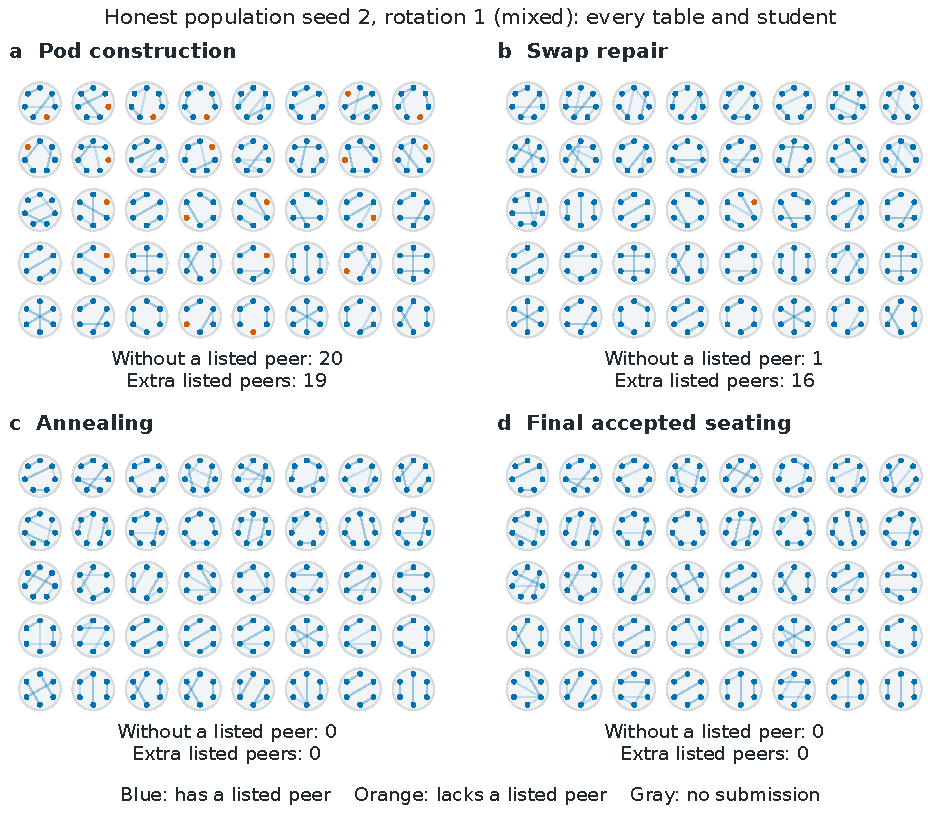
\includegraphics[width=\linewidth]{pipeline.pdf}
\caption{Actual optimization stages for honest population seed 2, rotation 1 (mixed). The four saved stage endpoints are actual assignments. Construction and repair can remain invalid; only a final chart that passes all hard-constraint checks is released.}\label{fig:pipeline}
\end{figure}

\subsection{Construction and repair}
Construction prioritizes participants with few supporting options, forms mutually compatible pods when possible, never pools a prohibited pair, and merges pods using compatibility and history scores without exceeding the minimum occupancy target. Pods are packed into admissible tables; packing failures can require singleton placement. The constructed chart meets every occupancy target but need not satisfy every companion obligation.

Repair uses directed exchanges and compound moves that close supporting dependencies. It attempts to reduce the unsatisfied set without orphaning a previously supported participant or creating another hard violation; a compound repair is kept only when the prescribed violation and cost checks succeed. A failed local repair does not imply infeasibility. Construction followed by repair, with the validated fallback of Section~\ref{sec:fallback} and no further optimization, is the companion-preserving baseline of the evaluation.

\subsection{Closure-preserving simulated annealing}
Let $\nu$ count unmet companion obligations, prohibited co-seatings, and placement-restriction violations scored by the search. Roster placement, occupancy, and grade eligibility are maintained as move invariants and are checked separately by the release validator; a zero search penalty alone is not a full validity certificate. The search uses the integer energy
\begin{equation}
 E=sC_r+1000s\,\nu,
\end{equation}
which is $10C_r+10000\nu$ for the default weights. The finite violation penalty is not itself a proof that a returned solution satisfies the guarantee. The acceptance filter separately requires $\Delta\nu\le0$, and the best assignment is retained lexicographically by violations and cost. Once $\nu=0$, accepted moves cannot break the guarantee. Before feasibility is reached, the total violation count can remain unchanged even if the identities of unsatisfied participants change.

The proposal mix uses uniform swaps, directed moves, and two-table group moves with probabilities $1/4$, $1/4$, and $1/2$. Group moves close supporting dependencies, balance table sizes, and retry bounded padding choices; placement restrictions filter proposals. During infeasible search, targeted proposals occur every eight iterations and compound repair attempts every 64. Costs are recomputed on affected tables, including all historical pair weights. A proposal passing the hard acceptance filter is accepted with probability $\min(1,\exp(-\Delta E/T))$. Temperature decreases from $2.5s$ to $0.02s$ over the specified budget, normally 300,000 iterations. This is a finite heuristic; no asymptotic convergence claim is used.

\subsection{Constraint programming on the exact objective and the acceptance guard}\label{sec:cp}
For present participant $i\in V_r$ and admissible table $t$, binary $x_{it}$ denotes assignment; variables for inadmissible tables are interpreted as zero. Exact-one constraints and $\sum_i x_{it}=o_t$ enforce placement and occupancy targets; prohibited pairs add $x_{at}+x_{bt}\le1$. Binary supporting indicators $y_{it}$ satisfy
\begin{equation}
 y_{it}\le x_{it},\qquad y_{it}\le\sum_{j\in L_i^{(r)}}x_{jt},\qquad\sum_t y_{it}\ge1\quad(i\in U_r).
\end{equation}
For each active obligated participant $i\in U_r$ with $\ell_i=|L_i^{(r)}|\ge2$, an integer variable $e_i\in\{0,\ldots,\ell_i-1\}$ counts listed peers beyond the first through
\begin{equation}
 e_i\ge\sum_{j\in L_i^{(r)}}x_{jt}-1-\ell_i(1-x_{it})\qquad(t\in\mathcal T_r).
\end{equation}
For $\ell_i=1$, set $e_i=0$. Let $H_r$ contain every unordered pair of present participants with nonzero history cost $h_{ab}=s\lambda(5m_{ab}+2\alpha_{ab})$, whether or not the pair met in the immediately preceding rotation. For these pairs, a binary variable $q_{ab}$ satisfying $q_{ab}\ge x_{at}+x_{bt}-1$ over tables marks a repeated meeting. CP-SAT minimizes
\begin{equation}\label{eq:cp}
 s\,w_e\sum_{i\in U_r}e_i+\sum_{\{a,b\}\in H_r}h_{ab}\,q_{ab},
\end{equation}
which for the default weights is $10\sum_i e_i+\sum_{\{a,b\}\in H_r}(5m_{ab}+2\alpha_{ab})q_{ab}$. For every valid chart the minimum over the auxiliary variables equals $sC_r$; the objective can overestimate a feasible but not proven optimal solution and can never underestimate it. Every returned chart is therefore rescored independently from its tables: the recomputed cost must not exceed the solver's objective, must equal it at OPTIMAL, and a violation of either comparison is treated as an implementation error. The hint is the better of the annealed chart and the validated incumbent; an invalid incumbent does not become a valid hint merely by being supplied to the solver. A CP candidate replaces a valid incumbent only if it is valid and does not worsen the independent score; if the incumbent is invalid, validity takes priority. The default improvement budget is 3.5 deterministic-time units with eight workers, and an OPTIMAL status is a proof of rotation optimality under the exact objective.

The historical surrogate, which counted participants with two or more listed peers and considered only the preceding rotation's pairs, is retained solely as an explicit option for comparison. An exploratory summary compares formulations on the same annealed incumbents of a 257-participant partial year (\BenchRotations\ rotations, \BenchAnnealIters\ annealing iterations, 3.5 deterministic units, up to \BenchMaxHistoryPairs\ weighted history pairs), the summary reports that the exact model took \BenchExactMeanSeconds\ s of wall time per rotation on average (maximum \BenchExactMaxSeconds\ s) against \BenchSurrogateMeanSeconds\ s for the surrogate, improved the incumbent in \BenchExactImproved\ rotations and worsened it in \BenchExactWorsened, whereas the surrogate's returned charts were worse under the full objective in \BenchSurrogateWorsened\ rotations and would have been rejected by the guard. The benchmark retained aggregate scores and timings, but no returned charts or source fingerprint, so these measurements cannot receive the independent trace checks applied to the primary study. They are preliminary performance evidence. The exact model is the default because it represents the stated objective.

If annealing remains infeasible, it permits up to six repair-and-anneal retries, each with $\max(I/2,20000)$ iterations for initial budget $I$, then a restart from the validated incumbent if one exists. If the guarded result remains infeasible, a final CP attempt uses $6\max(b,1)$ deterministic-time units for improvement budget $b$; if it cannot obtain a valid chart, the validated fallback is released with status \emph{fallback}, and if no fallback exists the rotation reports an unknown outcome instead of releasing a chart. An INFEASIBLE status is the solver's proof of model infeasibility; this project does not archive a separately checkable infeasibility proof object. Every released chart is checked for unique placement of the present roster, occupancy targets, eligibility, staff constraints, and all present obligations. Construction, repair, annealing, and final assignments, their costs, and their elapsed times are retained for inspection.

\section{Information revealed by published charts}\label{sec:privacy}
A public chart can reveal private list entries even when the lists themselves are hidden. We analyze an observer who knows that participant $i$ submitted a fixed list, knows a public upper bound $K$, knows the guarantee was honored, and observes all published charts. Let $T_i^{(r)}$ be the set of $i$'s tablemates in rotation $r$. Write $\mathcal R_i$ for observed rotations in which $i$ is present and has an unwaived obligation, assumed known to this observer. Only those rotations impose a guarantee constraint. Every candidate list $A$ must satisfy
\begin{equation}\label{eq:hit}
 |A|\le K,\qquad A\cap T_i^{(r)}\ne\varnothing\quad(r\in\mathcal R_i).
\end{equation}
A name $v$ is forced if excluding $v$ makes these hitting-set constraints impossible under the cap. An exact dynamic program over covered-rotation bitmasks computes minimum hitting-set sizes. An independent CP-SAT set-cover formulation checks the resulting exclusion certificates.

The production inference uses the public cap, not the private true list length. The assumed-public submitter identities are obtained from the input. Actual positive list entries are consulted only afterward to score correctness and the fraction of directed entries recovered. Recovering every true positive entry does not generally determine the entire list: additional names may still fit below the public cap. A list is uniquely determined by forced positives only when those positives fill the public cap, or fill an independently known exact list length. Exhausting the possible peer universe is another sufficient uniqueness condition; this degenerate case does not arise in the study. The output distinguishes complete true-positive recovery from uniquely determined lists.

Under this observer model, no individual name is forced in the first $K$ rotations when every observed table has at least three members. After excluding any one name, each tablemate set remains nonempty; choosing one remaining peer per rotation gives a hitting set of size at most $R\le K$. This explains the initial flat portion of the leakage curve, and it also describes a retention policy: an observer who keeps at most $K$ consecutive charts cannot force an individual entry. It does not mean that charts reveal no information: they already restrict the set of possible lists even without forcing an individual entry, and an observer who archives every chart privately is not bound by the school's retention policy.

Removing the public cap removes logical forcing altogether (any tablemate set of size at least two admits a hitting set avoiding a given name) but not statistical inference. The implementation therefore also reports the co-seating exposure: the fraction of obligated participants whose most frequent tablemate over the observed charts is a listed peer, for the proposed and for the matched random charts. This statistic needs no public cap but does require observations across rotations. It can be maintained with running co-seating counts instead of retaining the full charts; distributing only the current chart does not erase an observer's prior counts. Hiding lists, limiting archives, or removing a cap does not guarantee confidentiality, and the product reflects this: the student-facing export contains the assignment of one rotation and nothing else, history is an explicit opt-in, the full trace is a staff record, the static demonstration site has no access control, and the infrastructure a private distribution would need is documented as missing. A draft submission notice and data-handling policy state these limits to participants. This observer model omits some possible side information, and the system provides no formal privacy guarantee.

\section{Experimental design}\label{sec:design}
\subsection{Synthetic population and admission policy}
The reference population has 257 participants: 132 in grade 11 and 125 in grade 12. Forty tables contain 17 groups of seven and 23 groups of six. Same-grade rotations allocate twelve seven-seat and eight six-seat tables to grade 11, and five seven-seat and fifteen six-seat tables to grade 12. Sixteen rotations alternate mixed-grade and same-grade states, starting mixed.

A directed synthetic network targets up to eight true nominations per participant, using lognormal popularity, a within-grade weight, and reciprocal-edge generation. The reference regime reaches eight names; small latent groups at $\mu=1$ can yield shorter lists. Optional latent groups alter within-group preference and overlap. These parameters are scenario assumptions, not estimates from a school network. A six-person mutual clique is planted for attack comparisons, within one junior latent group when groups are enabled. The shared-anchor experiment adds a deterministic seventh coalition member and changes submitted lists while retaining the underlying population. Generated lists are classified into the submission states of Section~\ref{sec:model}; in the retained primary study every list was accepted (\PendingReview\ pending, \ApprovedExceptions\ approved exceptions, \VoluntaryNonsubmission\ voluntary nonsubmission), so the primary study supplies no outcomes for excluded or reviewed participants. The incomplete method comparison of Section~\ref{sec:evaldesign} includes some of those conditions, with coverage reported explicitly.
\begin{table}[tb]\centering\small
\caption{Reference configuration. Complete generator, submission, and solver configurations are retained in every trace.}\label{tab:params}
\begin{tabular}{@{}lp{9.2cm}@{}}\toprule
Parameter & Value \\ \midrule
Population & 257 (132 grade 11; 125 grade 12) \\
Tables & 17 $\times$ 7 and 23 $\times$ 6 \\
Rotations & 16, alternating mixed and same grade \\
Defended study lists & None or 4--8 names; at least 2 same grade \\
Reference nonsubmitters & 0 \\
Popularity / within-grade weight & $\sigma=0.6$ / 9 \\
Reciprocity target / realized & 0.5 / 0.490 \\
Realized within-grade fraction & 0.904 \\
Reference communities & $\mu=0,\ \omega=0$ \\
Annealing budget / temperature & 300,000 iterations / $25\to0.2$ (integer energy) \\
CP budget / workers & 3.5 deterministic-time units / 8 \\
Pre-feasibility budget & 20.0 deterministic-time units per state \\
Runtime versions & \Versions \\
\bottomrule\end{tabular}\end{table}


\subsection{Scenarios and structural attack score}
The six website reference scenarios share population seed seven: honest submission; an undefended one-name coalition cycle; a six-person four-of-five omission star; a six-person same-grade attack; the seven-person shared-anchor attack; and the six-person attack followed by the specified screened resubmission. The shared-anchor charts are deliberately generated with screening disabled, while a diagnostic records what the revised screen would return. A seventh scenario, a five-member mutual core with ten followers who list only the core, is a known infeasible input used by the method comparison; it is not on the website because nothing is scheduled.

For a coalition of size $q$, the member-weighted cluster size is
\begin{equation}
 H=\frac{1}{q}\sum_{G}|G\cap C|^2.
\end{equation}
An intact count records rotations with all coalition members together. For $q=6$, all six together may share a seven-seat table with an outsider; this is distinct from capturing a full table. The seven-member coalition fills a maximum-size table when intact.

In the omission-star wiring, every member lists four of the other five, and no one lists the central omitted member. Its feasible internal partition patterns are $3+3$, $4+2$, and $6$, with $H=3$, $10/3$, and $6$. The minimum $H=3$ is a structural lower bound on any valid outcome, not a prediction that every outcome has two triples. Exhaustive enumeration of $5^5$ wirings after fixing one omitted name gives the best lower bound \StarBound\ among that restricted internal six-person family. It does not optimize larger, externally anchored, or adaptive coalitions.

\subsection{Paired random baseline and metrics}
Each proposed schedule is compared with independently randomized seat permutations using the same occupancy targets, grade restrictions, and present population. This random comparator does not enforce companion obligations, staff-prohibited pairs, or individual placement restrictions; it is therefore not a feasible alternative when such constraints matter. For a uniform random rotation among $n\ge2$ present participants in one eligibility block, a particular pair meets with probability
\begin{equation}
 q_r=\frac{\sum_t o_t(o_t-1)}{n(n-1)}.
\end{equation}
The sum uses the block's occupancy targets, which can differ from physical capacities under absence. A pair has probability zero if either participant is absent or they are in different blocks. Independence across randomized rotations gives expected distinct peers by summing $1-\prod_r(1-q_{ab,r})$ over peers. For a participant with $k_i$ present eligible names at a table of actual occupancy $c$, random companion coverage is
\begin{equation}
 1-\frac{\binom{n-1-k_i}{c-1}}{\binom{n-1}{c-1}},
\end{equation}
averaged over table sizes with seat-share weights and over submitters. In the reference population, expected random coverage is \RandomGeOneExpectedMixed\% in mixed rotations and \RandomGeOneExpectedSame\% in same-grade rotations. Expected final distinct peers are \RandomMetExpected\ for the alternating schedule; the all-mixed value \RandomMetExpectedAllMixed\ is a different design and is not the applicable comparator.

Coverage and exactly-one percentages use present participants with unwaived obligations as the denominator. Distinct-peer means use all participants. Individual outcomes are recorded per participant for both the proposed and the random charts: distinct peers (with minimum and lower percentiles), extra listed companions, the maximum number of rotations spent with the same listed peer, and the share of obligated rotations spent with the most frequent listed peer. Repeat-pair counts count previously encountered unordered pairs in the current chart; they are not the weighted history cost in Equation~\eqref{eq:cost}. Coalition metrics use the actual scenario size. None of these statistics measures wellbeing: an unlisted tablemate is not assumed to be unfamiliar, and exactly-one coverage is an optimization statistic.

\subsection{Study plan, evidence, and uncertainty}
The primary comparison uses population seeds 1--10, each with honest and omission-star scenarios at the default budget and 16 rotations. Four additional seed-seven scenarios supply the remaining website references. Sensitivity runs vary annealing budgets to 100,000 and 900,000 iterations, CP budgets to 0.1 and 1.0 deterministic-time units, horizons to 5 and 32 rotations, and latent-group settings to $(\mu,\omega)=(0.6,0.3)$ and $(1,0)$. Each sensitivity changes its named setting relative to the seed-seven honest reference; it is not a factorial exploration. Population seeds and solver seeds are separate recorded fields.

\subsubsection*{Method comparison}\label{sec:evaldesign}
The revised implementation is also compared with a companion-preserving baseline, construction and repair with the validated fallback and no diversity optimization, on common populations, capacities, eligibility, and attendance inputs. The planned grid comprised population seeds 1--3, with a second solver seed for the reference condition, under eleven conditions: honest lists of up to eight names; generated lists truncated to four names, with approved exceptions where the rule fails; three-name lists, all approved exceptions; isolated latent communities ($\mu=1$); one quarter voluntary nonsubmission; a six percent synthetic absence rate with recorded waivers for unavoidable conflicts; the omission star; the shared-anchor attack; the known infeasible demand core with a 240-unit feasibility budget; honest lists with tiny feasibility and CP budgets; and the infeasible core with a tiny feasibility budget. The planned defaults were 100,000 annealing iterations, a CP budget of 1.0, and a feasibility budget of 10 unless a condition set its own; some retained retries used different feasibility budgets. Each job requests a full-year run in the same ledger, and the matched random charts are computed inside each run on the same present roster and targets. The retained grid is incomplete: 48 attempt records cover 44 of the 72 planned method configurations, with 31 successful traces, four review-required outcomes, four infeasible-input outcomes (two CP-SAT proofs for the demand core and two direct empty-eligible-list contradictions), five unknown outcomes, two interrupted attempts, and two attempts still marked running without terminal evidence. There are 15 matched configurations with successful traces for both methods; the remaining successful hybrid time-limited run has no successful counterpart. Most conditions cover only population seed one. Neither retained absence run required a waiver, so waiver handling is supported by regression tests rather than these empirical runs. Tables report all retained attempts and unpaired summaries of successful runs; their method averages need not use the same populations or retry budgets. The school's current procedure has no written rule specification available to us; the comparison is therefore against the matched random baseline and the construction-and-repair baseline, and this limitation is stated rather than filled by assumption.

Every attempted run is written to an atomic ledger before execution. Successful rows retain complete chart traces, effective inputs, configuration, source-file hashes, dependency versions, the full Git commit, and dirty-tree status. Interrupted, invalid, failed, review-required, proven infeasible, and unknown attempts remain visible. Resumption requires matching effective source and configuration identity and verified trace hashes. Table~\ref{tab:ledger} reports actual attempts. The study of 8 September 2026, produced by the previous implementation, is retained separately as historical evidence and excluded from the tables below; primary-study and evaluation numbers come from retained runs of the 11 September source (effective hash \SourceHash\ldots). The exploratory CP benchmark is separately identified as summary-only evidence. Subsequent audit repairs are covered by new regressions and independent rechecks; these traces are not fresh runs of the repaired source.
\begin{table}[tb]\centering\small
\caption{Attempt-level evidence inventory. Interrupted processes remain in the denominator after resumption; they do not establish either model infeasibility or solver failure. Other terminal outcomes, if any, are detailed in the machine-readable ledger.}\label{tab:ledger}
\begin{tabular}{@{}lrrrr@{}}\toprule
Experiment family & Attempts & Success & Interrupted & Other \\ \midrule
Primary population pairs & 20 & 20 & 0 & 0 \\
Additional reference attacks & 4 & 4 & 0 & 0 \\
Annealing sensitivity & 2 & 2 & 0 & 0 \\
CP sensitivity & 2 & 2 & 0 & 0 \\
Horizon sensitivity & 2 & 2 & 0 & 0 \\
Community sensitivity & 5 & 2 & 3 & 0 \\
\bottomrule\end{tabular}\end{table}


Population seeds, rather than students or rotations, are the independent units for paired comparisons. Reported ranges and a 95\% paired-population bootstrap percentile interval (20,000 resamples, PCG64 seed 20260908, linear sample quantiles) describe variation under this generator, conditional on the budgets and fixed study design; they are not uncertainty intervals for a real school population. Runtime measurements were collected with concurrent experiments on a shared machine and are not isolated hardware benchmarks.

\section{Results}\label{sec:results}
\subsection{Guarantee satisfaction, release statuses, and contact diversity}
All successful charts included in the results pass independent checks of placement, occupancy targets, eligibility, staff constraints, and the companion guarantee. This is a statement about retained, validated outputs; it is not evidence that every rule-compliant input is feasible or that every attempt succeeds. Across the \PrimaryRotations\ primary rotations, \ReleaseOptimized\ released a chart produced by that rotation's search, \ReleaseIncumbent\ released a validated cached chart that no search result beat, and \ReleaseFallback\ released the fallback because the search reached no valid chart of its own; construction and repair alone left \ConstructionInfeasibleRotations\ rotations infeasible before annealing. CP-SAT returned a feasible chart in \CpsatFeasibleRotations\ rotations, was accepted in \CpsatAcceptedRotations, and proved optimality under the exact objective in \ProvenOptimalRotations; the largest exact model carried \CpsatPairVarsMax\ weighted history pairs and \CpsatConstraintsMax\ constraints. In the seed-seven honest reference the CP stage took \CpsatMeanSeconds\ s of a \MeanSolveSeconds\ s mean rotation.

Across \NSeeds\ honest population seeds, mean exactly-one coverage is \SeedExactlyOneMean\%, with population means ranging from \SeedExactlyOneMin\% to \SeedExactlyOneMax\%. The paired change in final distinct peers averages \SeedDiffMean, ranging from \SeedDiffMin\ to \SeedDiffMax; the conditional 95\% bootstrap interval for the mean is [\SeedDiffCILow, \SeedDiffCIHigh].
\begin{table}[tb]\centering\small
\caption{Six verified seed-seven reference scenarios. Minimum guarantee and mean exactly-one rates are percentages of submitters; distinct contacts average over all participants. Intact and cluster values use the actual coalition size $q$.}\label{tab:summary}
\begin{tabular}{@{}lrrrrrr@{}}\toprule
Scenario & $q$ & $\ge1$ & Exactly 1 & Contacts & Intact & $H$ \\ \midrule
Honest & -- & 100 & 99.73 & 74.48 & -- & -- \\
One-name cycle & 6 & 100 & 99.73 & 72.86 & 16/16 & 6.00 \\
Omission star & 6 & 100 & 98.25 & 74.14 & 0/16 & 3.00 \\
Stratified attack & 6 & 100 & 98.52 & 73.58 & 8/16 & 3.71 \\
Shared-anchor attack & 7 & 100 & 99.29 & 72.72 & 8/16 & 4.71 \\
Screened resubmission & 6 & 100 & 98.25 & 74.14 & 0/16 & 3.00 \\
\bottomrule\end{tabular}\end{table}

\begin{table}[tb]\centering\small
\caption{Primary population comparisons at the default budget. Exactly-one percentages, distinct contacts (proposed and random), their paired difference, forced directed list entries, and the omission-star mean cluster size are computed from full traces.}\label{tab:seeds}
\begin{tabular}{@{}rrrrrrr@{}}\toprule
Seed & Exactly 1 & Contacts & Random & $\Delta$ & Forced & Star $H$ \\ \midrule
1 & 99.61 & 74.54 & 71.55 & +2.99 & 645 & 3.00 \\
2 & 99.54 & 74.71 & 72.25 & +2.46 & 642 & 3.00 \\
3 & 99.68 & 74.87 & 71.95 & +2.92 & 625 & 3.00 \\
4 & 99.59 & 74.40 & 72.33 & +2.07 & 615 & 3.00 \\
5 & 99.76 & 74.72 & 72.58 & +2.14 & 648 & 3.00 \\
6 & 99.63 & 74.53 & 72.39 & +2.14 & 593 & 3.00 \\
7 & 99.73 & 74.48 & 72.31 & +2.17 & 618 & 3.00 \\
8 & 99.68 & 74.50 & 72.04 & +2.46 & 647 & 3.00 \\
9 & 99.63 & 74.63 & 72.08 & +2.55 & 643 & 3.00 \\
10 & 99.83 & 74.83 & 72.09 & +2.74 & 618 & 3.00 \\
\bottomrule\end{tabular}\end{table}


For the seed-seven honest reference, mean exactly-one coverage is \HonestExactlyOne\%, and its minimum rotation value is \HonestExactlyOneMin\%. Mean final distinct peers are \HonestMet\ under the proposed schedule and \RandomMet\ under the paired random schedule. Figure~\ref{fig:year} shows the full trajectory, while Figure~\ref{fig:population} shows population-level variation. The proposed schedule has more repeated pairs than its random comparator in \RepeatsWorseCount\ reference rotations (\RepeatsWorseRotations). An aggregate diversity improvement therefore does not imply a per-rotation dominance result, and exactly-one coverage is an optimization statistic rather than a measure of social benefit.

\begin{figure}[tb]\centering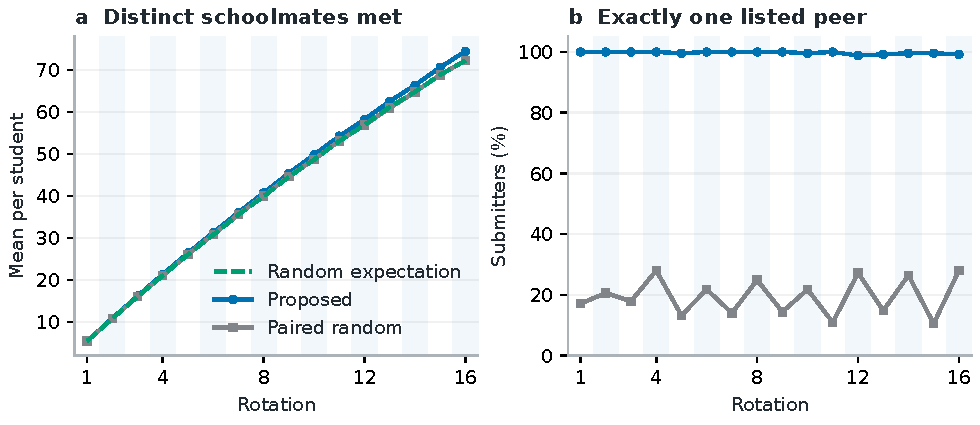
\includegraphics[width=\linewidth]{reference_year.pdf}
\caption{Seed-seven honest reference, using actual saved charts. Contact diversity is compared with the capacity- and eligibility-matched random schedule and its analytic expectation. Pale bands denote same-grade rotations. Companion statistics use submitters; contact diversity uses the whole population.}\label{fig:year}\end{figure}
\begin{figure}[tb]\centering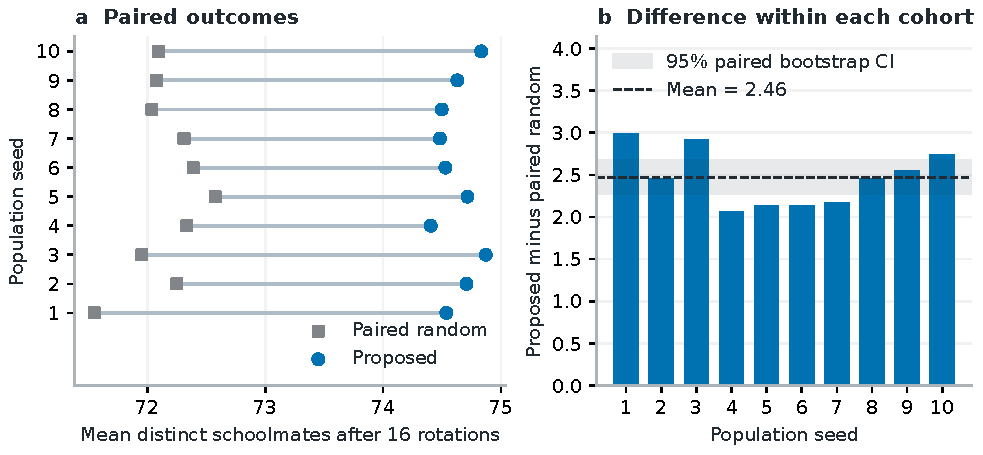
\includegraphics[width=\linewidth]{population_results.pdf}
\caption{Honest results across independent synthetic population seeds. Pairing preserves the population and eligibility schedule. The line and band in the difference panel show the paired mean and its 95\% population-bootstrap interval. They describe this synthetic design, not a sampled school population.}\label{fig:population}\end{figure}

\subsection{Individual outcomes}
In the seed-seven honest reference, individual final distinct-peer counts range from \FairMin\ to \FairMax, with a median of \PeersMedian\ and a 10th percentile of \PeersPTen\ (random: minimum \PeersMinRandom, 10th percentile \PeersPTenRandom). The per-participant maximum number of rotations with any one listed peer has median \RepeatSameMedian\ and maximum \RepeatSameMax, and the median share of obligated rotations spent with the most frequent listed peer is \ConcentrationMedian\%. Extra listed companions occurred at \ExtrasPerObligatedRotation\ per obligated participant-rotation. Participants in the lowest and highest incoming-nomination quartiles average \FairLowIn\ and \FairHighIn\ distinct peers, respectively. These descriptive statistics neither demonstrate equal treatment nor establish that nomination degree caused an outcome, and they omit satisfaction quality and the burden on participants with few acceptable peers; a pilot evaluation plan for those questions accompanies the repository, and no participant feedback is reported here.

\subsection{Coordinated submissions and screening}
The undefended cycle remains intact in \NoneIntact\ reference rotations. The omission star is intact in \StarIntact\ rotations and has mean cluster size \StarAvgCluster; observed patterns are \StarPatterns. These observations are compatible with all three feasible structural patterns in Figure~\ref{fig:structures}.

The six-person stratified attack remains intact in \StratIntactSame\ same-grade and \StratIntactMixed\ mixed-grade rotations. The seven-person shared-anchor attack remains intact in \SharedIntactSame\ same-grade rotations, consistent with Proposition~\ref{prop:shared}. The revised diagnostic returns \SharedReturned\ coalition members; it does not return the common anchor solely because it supports the proof. The screened six-person resubmission has mean cluster size \ScreenedAvgCluster\ and is intact in \ScreenedIntact\ rotations; its full-model tests examined \ScreenedFullModelExamined\ high-risk candidate groups of the replacement submission and certified \ScreenedFullModelForced\ as forced under the complete constraints. This one response illustrates changed behavior after a certified return, not complete strategic resistance. The shared-anchor run also has fewer room-wide distinct contacts than the common random baseline, despite satisfying every hard companion constraint. The honest-regime diversity gain therefore does not extend to every tested submission regime.
\begin{table}[tb]\centering\small
\caption{Reference screening by eligibility state. The initial screened attack and its replacement lists are separate rows: retained full-model tests use the replacement lists. Certificates may overlap and do not count distinct students. Target cores show examined/discovered bounded candidates. Full model shows examined/discovered tests, followed by forced/separable/unresolved counts. These are checks on the archived full-attendance states, not recall against all possible attacks.}\label{tab:screen}
\begin{tabular}{@{}llrrrl@{}}\toprule
Submission & State & Certificates & Unresolved & Target cores & Full model \\ \midrule
Honest & mixed & 0 & 0 & 0/0 & 0/0; 0/0/0 \\
Honest & same & 0 & 0 & 0/0 & 0/0; 0/0/0 \\
Shared-anchor attack & mixed & 0 & 0 & 0/0 & -- \\
Shared-anchor attack & same & 1 & 0 & 1/1 & -- \\
Initial screened attack & mixed & 0 & 0 & 0/0 & -- \\
Initial screened attack & same & 2 & 0 & 0/6 & -- \\
After resubmission & mixed & 0 & 0 & 5/6 & 5/5; 0/5/0 \\
After resubmission & same & 0 & 0 & 5/6 & 5/5; 0/5/0 \\
\bottomrule\end{tabular}\end{table}


\subsection{Method comparison}
Tables~\ref{tab:evalOutcomes} and~\ref{tab:evalQuality} summarize retained attempts for the hybrid and construction-and-repair methods. The incomplete grid and method-specific failures make these unpaired summaries; they are not a balanced estimate of the method difference. The outcome table reports each retained status, including unfinished attempts, and how often a rotation fell back to the validated cached chart; the quality table reports coverage, objective components, individual outcome distributions, and statistical exposure for scheduled runs, with the matched random baseline from the same runs. The infeasible condition demonstrates a proven infeasible outcome, and the time-limited conditions demonstrate that an UNKNOWN preliminary check neither blocks a later validated chart nor becomes a proof of infeasibility. These are descriptive comparisons on a few synthetic populations at a reduced budget; they identify trade-offs rather than establishing that either method is preferable for a real school.
\begin{table}[tb]\centering\scriptsize\setlength{\tabcolsep}{4pt}
\caption{The planned grid is incomplete; methods have unequal population, solver-seed, and retry coverage. Method comparison: retained attempt outcomes per condition. Scheduled means every rotation released an independently validated chart; review, infeasible and unknown are the explicit non-scheduled outcomes. Runtime is the mean wall-clock year time on a shared machine. Fallback counts rotations that released the unchanged validated fallback chart. Other includes interruptions and 2 attempts still marked running in the saved ledgers; these have no terminal outcome.}\label{tab:evalOutcomes}
\begin{tabular}{@{}llrrrrrrrr@{}}\toprule
Condition & Method & Att. & Sched. & Review & Infeas. & Unknown & Other & Year s & Fallback rot. \\ \midrule
absences & construct\_repair & 1 & 1 & 0 & 0 & 0 & 0 & 43 & 3.0 \\
absences & hybrid & 1 & 1 & 0 & 0 & 0 & 0 & 113 & 0.0 \\
coalition\_star & construct\_repair & 1 & 1 & 0 & 0 & 0 & 0 & 5 & 3.0 \\
coalition\_star & hybrid & 1 & 1 & 0 & 0 & 0 & 0 & 82 & 0.0 \\
concentrated & construct\_repair & 1 & 1 & 0 & 0 & 0 & 0 & 14 & 15.0 \\
concentrated & hybrid & 3 & 1 & 0 & 0 & 0 & 2 & 109 & 0.0 \\
infeasible & construct\_repair & 1 & 0 & 0 & 1 & 0 & 0 & -- & -- \\
infeasible & hybrid & 1 & 0 & 0 & 1 & 0 & 0 & -- & -- \\
nonsubmission & construct\_repair & 2 & 1 & 0 & 0 & 0 & 1 & 5 & 1.0 \\
nonsubmission & hybrid & 1 & 1 & 0 & 0 & 0 & 0 & 218 & 0.0 \\
reference & construct\_repair & 6 & 6 & 0 & 0 & 0 & 0 & 6 & 2.7 \\
reference & hybrid & 6 & 6 & 0 & 0 & 0 & 0 & 116 & 0.0 \\
shared\_anchor & construct\_repair & 1 & 1 & 0 & 0 & 0 & 0 & 5 & 10.0 \\
shared\_anchor & hybrid & 1 & 1 & 0 & 0 & 0 & 0 & 122 & 0.0 \\
short\_lists & construct\_repair & 3 & 3 & 0 & 0 & 0 & 0 & 6 & 16.0 \\
short\_lists & hybrid & 3 & 3 & 0 & 0 & 0 & 0 & 156 & 0.0 \\
three\_name\_lists & construct\_repair & 4 & 1 & 2 & 1 & 0 & 0 & 14 & 16.0 \\
three\_name\_lists & hybrid & 5 & 1 & 2 & 1 & 0 & 1 & 521 & 0.0 \\
time\_limited & construct\_repair & 1 & 0 & 0 & 0 & 1 & 0 & -- & -- \\
time\_limited & hybrid & 1 & 1 & 0 & 0 & 0 & 0 & 51 & 0.0 \\
time\_limited\_infeasible & construct\_repair & 2 & 0 & 0 & 0 & 2 & 0 & -- & -- \\
time\_limited\_infeasible & hybrid & 2 & 0 & 0 & 0 & 2 & 0 & -- & -- \\
\bottomrule\end{tabular}\end{table}

\begin{table}[tb]\centering\scriptsize\setlength{\tabcolsep}{4pt}
\caption{The planned grid is incomplete; methods have unequal population, solver-seed, and retry coverage. Unpaired summaries of scheduled runs: coverage among obligated students (\%), extra listed companions per obligated student-rotation, total unscaled objective over the year, distinct peers per student (mean; matched random mean; 10th percentile; minimum), median over students of the maximum number of rotations spent with the same listed peer, and the fraction of obligated students whose most frequent tablemate is a listed peer (statistical exposure). Means over runs.}\label{tab:evalQuality}
\begin{tabular}{@{}llrrrrrrrrrrr@{}}\toprule
Condition & Method & Runs & $\ge1$ & $=1$ & Extras & Obj. & Peers & Rand. & P10 & Min & Rep. & Exp. \\ \midrule
absences & construct\_repair & 1 & 100.0 & 91.0 & 0.095 & 1122.2 & 62.3 & 64.7 & 57.0 & 50 & 5.0 & 0.97 \\
absences & hybrid & 1 & 100.0 & 99.0 & 0.010 & 552.9 & 65.5 & 64.7 & 59.6 & 53 & 4.0 & 0.95 \\
coalition\_star & construct\_repair & 1 & 100.0 & 89.5 & 0.111 & 1668.9 & 66.9 & 71.5 & 63.0 & 51 & 5.0 & 0.94 \\
coalition\_star & hybrid & 1 & 100.0 & 98.0 & 0.020 & 749.2 & 73.7 & 71.5 & 70.0 & 59 & 4.0 & 0.96 \\
concentrated & construct\_repair & 1 & 100.0 & 57.2 & 0.608 & 17061.6 & 15.9 & 71.5 & 15.0 & 13 & 8.0 & 0.49 \\
concentrated & hybrid & 1 & 100.0 & 85.5 & 0.145 & 1087.7 & 75.5 & 71.5 & 72.0 & 67 & 4.0 & 0.95 \\
nonsubmission & construct\_repair & 1 & 100.0 & 97.6 & 0.025 & 738.0 & 76.6 & 71.5 & 71.0 & 67 & 5.0 & 0.97 \\
nonsubmission & hybrid & 1 & 100.0 & 99.8 & 0.002 & 428.1 & 77.9 & 71.5 & 73.0 & 69 & 4.0 & 0.97 \\
reference & construct\_repair & 6 & 100.0 & 91.0 & 0.093 & 1604.4 & 66.0 & 71.9 & 62.0 & 58 & 5.0 & 0.96 \\
reference & hybrid & 6 & 100.0 & 99.2 & 0.008 & 641.3 & 74.3 & 71.9 & 70.3 & 65 & 4.0 & 0.96 \\
shared\_anchor & construct\_repair & 1 & 100.0 & 86.1 & 0.145 & 9745.1 & 39.1 & 71.5 & 36.0 & 27 & 9.0 & 0.61 \\
shared\_anchor & hybrid & 1 & 100.0 & 98.6 & 0.014 & 1049.5 & 72.7 & 71.5 & 69.0 & 33 & 4.0 & 0.95 \\
short\_lists & construct\_repair & 3 & 100.0 & 92.5 & 0.079 & 18206.4 & 10.2 & 71.9 & 8.7 & 8 & 8.0 & 0.43 \\
short\_lists & hybrid & 3 & 100.0 & 96.7 & 0.034 & 2061.8 & 62.2 & 71.9 & 55.3 & 44 & 7.0 & 0.94 \\
three\_name\_lists & construct\_repair & 1 & 100.0 & 92.6 & 0.076 & 18398.4 & 10.1 & 72.0 & 9.0 & 8 & 8.0 & 0.42 \\
three\_name\_lists & hybrid & 1 & 100.0 & 96.8 & 0.033 & 4539.1 & 48.9 & 72.0 & 36.0 & 25 & 10.0 & 0.86 \\
time\_limited & hybrid & 1 & 100.0 & 99.2 & 0.008 & 654.8 & 74.1 & 71.5 & 70.0 & 63 & 4.0 & 0.98 \\
\bottomrule\end{tabular}\end{table}


\subsection{Budget and network sensitivity}
Table~\ref{tab:sensitivity} and Figure~\ref{fig:sensitivity} vary computational budgets, horizon, and latent network structure. A larger budget changes a finite search opportunity; it need not monotonically improve every downstream-year metric. The $\mu=1,\omega=0$ latent-group setting has exactly-one coverage \IsolatedExactlyOne\%, compared with \HonestExactlyOne\% in the reference. Network concentration can therefore substantially change the apparent ability to minimize extras. At $\mu=1$, smaller groups also shorten realized lists (mean \IsolatedMeanList\ names rather than eight), so this comparison changes both network concentration and the list-length distribution. It is not an isolated causal estimate of community structure. One-population sensitivity runs identify dependence on assumptions but cannot establish general robustness.
\begin{table}[tb]\centering\small
\caption{Seed-seven honest sensitivity, with one setting changed at a time. Contact counts and forced entries depend on horizon and should be compared at equal horizons. "No list" counts voluntary nonsubmission and pending requests; it is distinct from an unmet seating guarantee. "Cached" counts rotations that released a validated cached chart (incumbent or fallback) rather than a chart produced by that rotation's search.}\label{tab:sensitivity}
\begin{tabular}{@{}lrrrrrrr@{}}\toprule
Setting & $R$ & Exactly 1 & Contacts & Random & Forced & No list & Cached \\ \midrule
Reference (16 rotations) & 16 & 99.73 & 74.48 & 72.31 & 618 & 0 & 0 \\
Anneal 100,000 & 16 & 99.34 & 74.42 & 72.31 & 576 & 0 & 0 \\
Anneal 900,000 & 16 & 99.76 & 74.98 & 72.31 & 705 & 0 & 0 \\
CP budget 0.1 & 16 & 99.68 & 74.54 & 72.31 & 602 & 0 & 0 \\
CP budget 1 & 16 & 99.71 & 74.66 & 72.31 & 612 & 0 & 0 \\
Horizon 5 & 5 & 99.92 & 26.45 & 26.15 & 0 & 0 & 0 \\
Horizon 32 & 32 & 99.28 & 129.14 & 120.44 & 1648 & 0 & 0 \\
Groups $\mu=0.6,\omega=0.3$ & 16 & 99.54 & 75.03 & 72.31 & 583 & 0 & 0 \\
Groups $\mu=1,\omega=0$ & 16 & 89.59 & 75.62 & 72.31 & 534 & 0 & 0 \\
\bottomrule\end{tabular}\end{table}

\begin{figure}[tb]\centering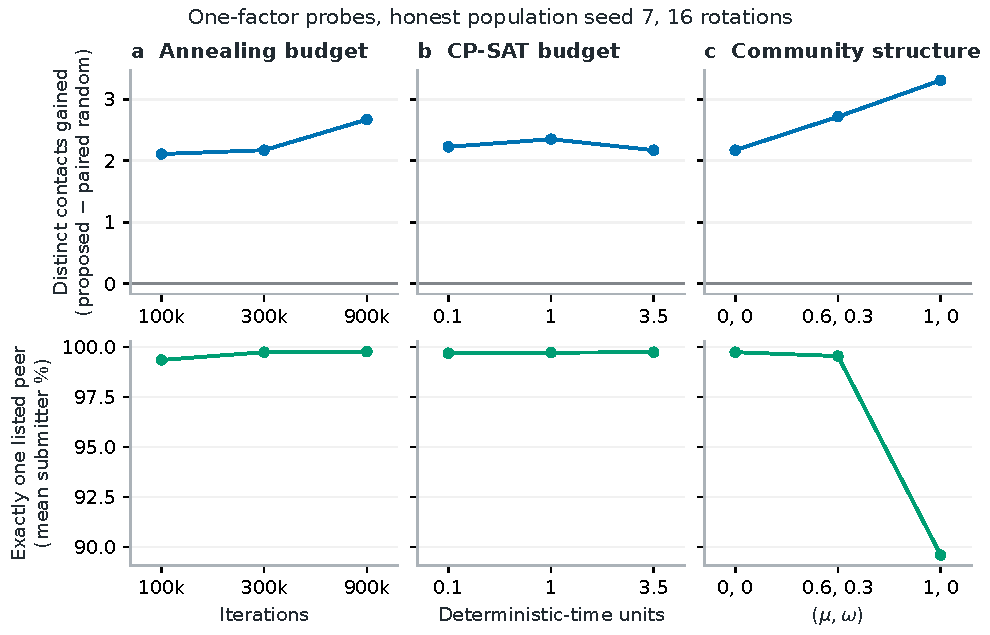
\includegraphics[width=\linewidth]{sensitivity.pdf}
\caption{Sensitivity of the seed-seven honest scenario to annealing effort, CP improvement budget, and latent community structure. Other settings use the reference values. Each point represents a single generated population and finite solver run; these are descriptive comparisons.}\label{fig:sensitivity}\end{figure}

\subsection{Privacy implications}
In the reference run, the public-cap inference forces \LeakForced\ of \LeakEdges\ directed submitted entries (\LeakFraction\%), affecting \LeakStudents\ participants. Comparison with private synthetic truth confirms \LeakCorrect\ forced entries as correct. Ties in co-seating frequency are broken by ascending anonymous participant ID, for both methods. The inference classifies \LeakFull\ lists as uniquely determined under the public cap; this count is separate from complete recovery of a shorter true list. Figure~\ref{fig:privacy} displays the accumulation of forced entries and the distribution of distinct contacts.

The 32-rotation sensitivity forces \LongLeakForced\ directed entries (\LongLeakFraction\%) and uniquely determines \LongLeakFull\ lists under the public cap. The five-rotation probe forces no entries, as predicted by the preceding hitting-set argument, and distributing only the current chart forces \CurrentOnlyForced\ entries at any point of the reference year. Statistical exposure is another matter: the most frequent tablemate of an obligated participant is a listed peer for \ExposureTopOne\% of participants under the proposed charts (\ExposureTopThree\% of the three most frequent tablemates), against \ExposureTopOneRandom\% under the matched random charts. The most-frequent rank is tied for 91 proposed-chart participants and 153 random-chart participants. Across all possible choices within those ties, the listed-peer rate ranges from 93.4\% to 98.8\% for the proposed charts and from 1.6\% to 12.5\% for random charts; the reported point estimates use the stated ID rule. These are one-population comparisons under fixed submissions; they do not imply that every population has the same disclosure rate, but they do show that neither hiding lists, nor limiting the archive, nor removing a public cap guarantees confidentiality.
\begin{figure}[tb]\centering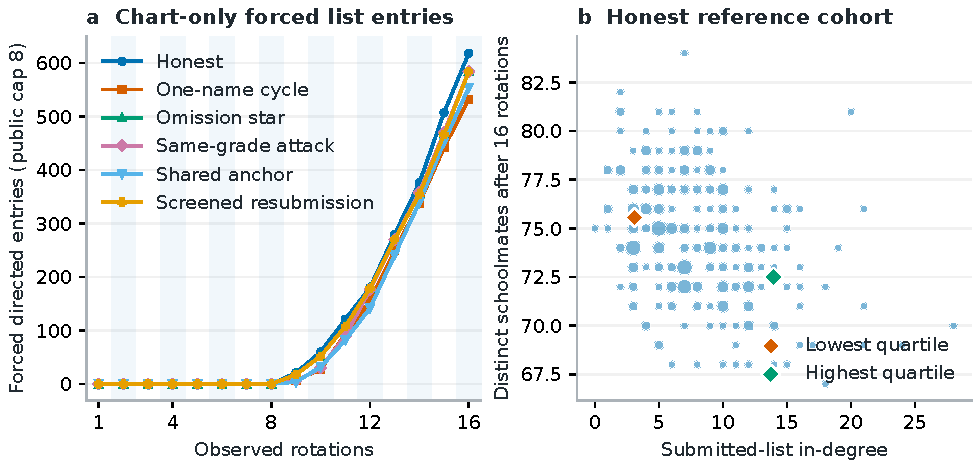
\includegraphics[width=\linewidth]{leakage_fairness.pdf}
\caption{Information implied by successive published charts under the stated public cap across the six reference scenarios (left), and individual contact diversity by incoming nomination degree in the honest reference population (right). Private truth scores inference afterward; it is not supplied to the observer. Pale bands denote same-grade rotations; larger scatter markers combine students at identical coordinates. The degree association is descriptive.}\label{fig:privacy}\end{figure}

\section{Discussion and limitations}
The strongest guarantees in this work are local and explicit: every released chart satisfies the stated constraints, every certified targeted core is forced together under the relaxation's hypotheses, every full-model forcing test excludes a separating valid chart under the complete current constraints, with nonvacuous forcing conditional on base feasibility, and every fallback chart was validated before release. These statements do not imply that the screen detects every forceable coalition. Single-anchor deletion, a bounded core size, and a budgeted number of full-model tests target useful counterexamples, but multiple anchors, larger cores, and adaptive submissions remain outside an exhaustive analysis. A screen passage means only that the implemented checks did not certify a problem. A proved-coercive or forced structure does not establish dishonest intent, and recurring co-seating is reported as a diagnostic, not as a finding.

Global feasibility remains a distinct question. Feasibility certificates concern the specified occupancy targets as well as physical capacities. The largest-first attendance rule can create singleton targets even when a different allocation of the same physical seats would admit a valid chart; target selection is therefore an additional design limitation, and an infeasible fixed-target model need not imply that the physical room cannot seat the population. Minimum list length and two same-grade names do not imply it, and a time-limited unknown solve must not be described as a proof of failure; the outcome vocabulary of Section~\ref{sec:model} keeps proven infeasibility, unknown, review required, and scheduled apart. Where an instance needs review, an operational deployment needs the administrator workflow documented with the repository: decisions on pending requests, attendance conflicts, staff constraints, and manual adjustments, all validated against the same hard constraints. This study does not validate that process with real participants.

The objectives are operational proxies. Fewer extra listed peers and more distinct contacts may be useful design choices, and the penalty for extra companions is now configurable, but this study contains no intervention, calibrated friendship network, or measured wellbeing outcome, and it does not claim a socially optimal weight. The synthetic generator, planted coalition, public cap, and fixed budgets restrict external validity. The random and construction-and-repair baselines measure two particular alternatives; the school's current procedure could not be compared because its rules are not specified in writing. The study also lacks a full-year optimality certificate and extensive algorithmic ablations.

Publication of charts has a substantive privacy cost in the observer model, and statistical exposure is measurable without a cap when observers retain recurrence counts. The project should not be presented as privacy-preserving. The product-side measures, a chart-only student export, current-only distribution by default, and explicit policy drafts, limit what is distributed; they do not make the assignment confidential, and the static demonstration site has no access control. Any deployment would need an authenticated channel and a data policy that the school owns.

Source and input fingerprints improve auditability, but multiworker optimization and platform differences can still change search trajectories. The attempt ledger and independently validated trace are the evidence for each reported outcome. Historical proposal files describing maximization of two-friend coverage or all-mixed baselines are not the current specification, and the study of 8 September 2026 is historical evidence of a previous implementation rather than a result of this one. The original external prototype and collusion-result files described in earlier materials were not available; no claim of reproducing those historical experiments is made.

\section{Conclusion}
A hard companion guarantee creates both an assignment constraint and a strategic dependency structure. Shared outside anchors show why closure-only reasoning can miss full-table capture. A targeted relaxation and a full-model separation test yield sound forcing certificates for examined groups, while explicit unresolved states prevent time limits from masquerading as proofs. Explicit submission states, attendance-aware rosters, staff constraints, and validated fallback charts turn the ordinary frictions of a school into recorded decisions rather than silent changes. The implemented hybrid solver, with one canonical objective from annealing through constraint programming, produces independently validated synthetic schedules with high exactly-one coverage and modest gains in distinct contacts relative to a matched random baseline. Those gains coexist with preference disclosure under the specified observer model, which the studied distribution measures do not eliminate, and with unresolved questions about complete screening, real-world feasibility, and social outcomes.

\section*{Declarations}
\paragraph{Author and affiliations.} Isaac Lin; \AuthorAffiliations. The institutional labels were supplied by the author. The full institutional name represented by SMU and the final contribution statement must be confirmed before submission.
\paragraph{Funding.} \FundingDeclaration
\paragraph{Competing interests.} \ConflictDeclaration
\paragraph{Ethics and participants.} The reported experiments use synthetic participants and synthetic preference networks. No human-subject intervention or real student preference data are reported. No ethics approval for a future deployment is asserted.
\paragraph{Data and code availability.} The project repository is \url{https://github.com/IsaacLin247/lunch-seating-visual}. The interactive trace playback is at \url{https://isaaclin247.github.io/lunch-seating-visual/}. The revised evidence and corrected sources of this draft remain local and had not been deposited at those public links when checked on 13 September 2026; a versioned release containing them is required for submission. The retained attempt manifests identify the effective source and inputs of each experiment.
\paragraph{Acknowledgments.} Independent audit findings motivated the regression suite and the separation of mathematical certificates, heuristic outcomes, and empirical scope.

\bibliographystyle{unsrtnat}
\bibliography{refs}
\appendix
\section{Reproduction and independent verification}
The repository pins simulation dependencies in \texttt{requirements.txt} and figure dependencies in \texttt{requirements-paper.txt}. The exact fresh-study commands and concurrency conditions are documented in \texttt{results/STUDY.md}; every option is described in \texttt{CONFIGURATION.md}. The saved manifests include population and solver seeds separately, the complete generator, submission, attendance, staff-constraint, objective, and solver configuration, effective input hashes, full Git identity, dirty status, source-file fingerprints, and versions. A source fingerprint covers executable simulation files and simulation requirements, excluding generated figures, manuscript files, and outputs; the executable source of each study is archived byte for byte under its fingerprint. A dirty checkout is therefore identified explicitly rather than being mislabeled by a short commit alone.

\begin{lstlisting}[basicstyle=\ttfamily\footnotesize,breaklines=true]
python -m pip install -r requirements-paper.txt
python -m pytest -q
python paper/assemble_evidence.py --retained-source
python paper/assemble_evidence.py --retained-source --no-site --partial \
  --inputs results/revised_evaluation_a.json results/revised_evaluation_b.json \
  --out results/revised_evaluation.json
python paper/make_tables.py
python paper/make_evaluation.py --manifest results/revised_evaluation.json --retained-source
python paper/make_figures.py --retained-source
python results/verification/verify_traces.py \
  results/revised_experiments.json \
  --out results/verification/revised_charts.json
cd article
latexmk -pdf -interaction=nonstopmode article.tex
\end{lstlisting}
The assembler rejects unfinished inputs for a final study assembly and verifies saved hashes. The explicitly partial evaluation assembly preserves unfinished records, and its tables disclose incomplete coverage; this exception does not certify the planned grid as complete. The trace checker independently recomputes occupancy targets for present rosters, table feasibility, staff constraints, stage costs including hard violations and the unscaled objective, rotation statistics, release statuses and optimality claims, coalition patterns, distributional summaries, and aggregate results. A separate CP formulation checks privacy exclusion claims. The website receives the six completed seed-seven traces, including actual construction, repair, annealing, and final endpoints.

\section{Regression evidence and audit scope}
The 13 September regressions additionally cover empty attendance pools, rejection of phantom occupancy targets, independent validation when retaining fallbacks, actual-roster preflight, unresolved full-model review checks, configured screening budgets, waived-rotation privacy constraints, over-cap approval rejection, and student-export field minimization. These checks are separate from the archived experimental runs. The regression suite covers the 257-participant shared-anchor witness, restoration of anchor edges during targeted testing, exact senior capacity pools, unknown solver statuses, and the additional failure modes of this revision: a valid preliminary chart survives a forced failure of every optimization stage; a changed obligation changes the hard-constraint key and revalidation rejects the stale chart; short lists remain visible requests and approved exceptions keep their obligations; an absent sole companion produces an explicit conflict that only a recorded waiver resolves; the CP-SAT objective equals the independent score and the brute-force optimum on small instances; historical pairs omitted from the preceding rotation still incur their cost; the full-model test distinguishes validated separating witnesses, forced groups, and unresolved results; every released chart satisfies staff constraints, occupancy targets, and present obligations; and student-facing exports omit every private field. Exhaustive seating partitions of 180 small random graphs independently check that every certified core is forced together. These tests validate soundness on the enumerated cases; they do not prove completeness of candidate generation. The star enumeration checks all restricted four-of-five wirings and retains all feasible partition patterns. Privacy tests distinguish a recovered short list from a uniquely determined list under a public cap. Ledger tests preserve interrupted attempts, reject stale or modified traces, and bind resumption to matching source and configuration identity.

The accompanying audit-resolution document maps each finding, including the seven design findings addressed in this revision, to its correction or remaining limitation. Historical source documents and summary-only experiments are preserved as history. Their former objective and numbers are excluded from current claims rather than silently treated as fresh evidence.
\end{document}
